\documentclass[aspectratio=169, 10pt]{beamer}

% ── Encoding & fonts ──────────────────────────────────────────────────────────
\usepackage[T1]{fontenc}
\usepackage[utf8]{inputenc}
\usepackage{lmodern}
\usepackage{microtype}

% ── Math ──────────────────────────────────────────────────────────────────────
\usepackage{amsmath, amssymb}

% ── Graphics & colour ─────────────────────────────────────────────────────────
\usepackage{graphicx}
\usepackage{xcolor}
\usepackage{tikz}
\usetikzlibrary{arrows.meta, positioning, calc}

% ── Tables ────────────────────────────────────────────────────────────────────
\usepackage{booktabs}
\usepackage{array}
\usepackage{colortbl}

% ── Code listings ─────────────────────────────────────────────────────────────
\usepackage{listings}

% ── Misc ──────────────────────────────────────────────────────────────────────
\usepackage{hyperref}

% =============================================================================
%  COLOURS  (mirror report.tex palette)
% =============================================================================
\definecolor{aims-blue}{RGB}{0, 70, 127}
\definecolor{aims-teal}{RGB}{13, 124, 124}
\definecolor{aims-green}{RGB}{39, 174, 96}
\definecolor{aims-red}{RGB}{231, 76, 60}
\definecolor{aims-purple}{RGB}{142, 68, 173}
\definecolor{aims-orange}{RGB}{211, 84, 0}
\definecolor{aims-lblue}{RGB}{41, 128, 185}
\definecolor{code-bg}{RGB}{240, 244, 248}
\definecolor{code-red}{RGB}{192, 57, 43}

% =============================================================================
%  BEAMER THEME
% =============================================================================
\usetheme{default}
\usecolortheme{default}

% Colours
\setbeamercolor{normal text}{fg=black!85}
\setbeamercolor{structure}{fg=aims-blue}
\setbeamercolor{frametitle}{fg=white, bg=aims-blue}
\setbeamercolor{title}{fg=white, bg=aims-blue}
\setbeamercolor{block title}{fg=white, bg=aims-teal}
\setbeamercolor{block body}{fg=black!85, bg=aims-teal!8}
\setbeamercolor{alerted text}{fg=aims-teal}
\setbeamercolor{item}{fg=aims-blue}
\setbeamercolor{subitem}{fg=aims-teal}
\setbeamercolor{footline}{fg=white, bg=aims-blue}

% Fonts
\setbeamerfont{title}{size=\LARGE, series=\bfseries}
\setbeamerfont{frametitle}{size=\large, series=\bfseries}
\setbeamerfont{block title}{size=\small, series=\bfseries}
\setbeamerfont{footline}{size=\tiny}

% Frametitle: thin teal rule below the bar
\setbeamertemplate{frametitle}{%
  \vspace{0.25em}\insertframetitle%
  \ifx\insertframesubtitle\empty\else
    \\[0.05em]{\small\color{aims-teal!70!white}\insertframesubtitle}%
  \fi%
}

% No navigation icons
\setbeamertemplate{navigation symbols}{}

% Footer: project name left, slide counter right
\setbeamertemplate{footline}{%
  \begin{beamercolorbox}[wd=\paperwidth, ht=2.2ex, dp=1ex]{footline}%
    \hspace{1em}%
    AIMS RIC \textbullet\ DTS 2026 \textbullet\ ML-ESS%
    \hfill%
    \insertframenumber\,/\,\inserttotalframenumber%
    \hspace{1em}%
  \end{beamercolorbox}%
}

% Progress bar in headline (teal, grows with each slide)
\setbeamertemplate{headline}{%
  \begin{beamercolorbox}[wd=\paperwidth, ht=2pt, dp=0pt]{aims-teal}%
    \begin{tikzpicture}
      \useasboundingbox (0,0) rectangle (\paperwidth, 2pt);
      \pgfmathsetlength{\progressbarwidth}{\paperwidth * \insertframenumber / \inserttotalframenumber}
      \fill[aims-teal] (0,0) rectangle (\progressbarwidth, 2pt);
    \end{tikzpicture}%
  \end{beamercolorbox}%
}

% Itemize bullets
\setbeamertemplate{itemize item}{\small\color{aims-teal}$\blacktriangleright$}
\setbeamertemplate{itemize subitem}{\small\color{aims-blue}--}
\setbeamertemplate{enumerate item}{\color{aims-blue}\insertenumlabel.}

% Title page
\setbeamertemplate{title page}{%
  \begin{center}
    \vfill
    {\usebeamerfont{title}\color{aims-blue}\inserttitle}\par
    \vspace{0.4em}
    {\large\color{aims-teal}\insertsubtitle}\par
    \vspace{0.6em}
    \textcolor{aims-teal}{\rule{5cm}{1pt}}\par
    \vspace{0.6em}
    {\normalsize\insertauthor}\par
    \vspace{0.4em}
    {\small\color{black!55}\insertinstitute}\par
    \vspace{0.4em}
    {\small\color{aims-blue}\insertdate}
    \vfill
  \end{center}%
}

% =============================================================================
%  CODE LISTINGS
% =============================================================================
\lstdefinestyle{pycode}{
  language=Python,
  backgroundcolor=\color{code-bg},
  basicstyle=\ttfamily\scriptsize,
  keywordstyle=\color{aims-blue}\bfseries,
  stringstyle=\color{aims-green!80!black},
  commentstyle=\color{black!45}\itshape,
  identifierstyle=\color{black!85},
  breaklines=true,
  showstringspaces=false,
  frame=single, framerule=0.4pt, rulecolor=\color{aims-blue!25},
  xleftmargin=0.5em, xrightmargin=0.5em, framexleftmargin=0.4em,
  aboveskip=0.3em, belowskip=0.2em,
}
\lstdefinestyle{shcode}{
  language=bash,
  backgroundcolor=\color{black!90},
  basicstyle=\ttfamily\scriptsize\color{white!85},
  breaklines=true, showstringspaces=false,
  frame=none, xleftmargin=0.5em,
  aboveskip=0.3em, belowskip=0.2em,
}

% =============================================================================
%  HELPER MACROS
% =============================================================================

% Inline mono/code
\newcommand{\code}[1]{{\ttfamily\small\color{code-red}#1}}

% Teal highlight box (uses beamer block)
\newenvironment{hlbox}{%
  \begin{beamercolorbox}[rounded=true, sep=4pt, wd=\linewidth]{block body}%
    \small}{%
  \end{beamercolorbox}}

% Amber note box
\newenvironment{notebox}{%
  \vspace{0.2em}%
  \noindent\colorbox{yellow!18}\bgroup\parbox{\dimexpr\linewidth-2\fboxsep\relax}{\tiny\color{black!70}%
}{%
  \par}\egroup\vspace{0.1em}%
}

% Simpler note: \note{text}  (no environments)
\newcommand{\sidenote}[1]{%
  \vspace{0.2em}%
  \noindent\colorbox{yellow!18}{%
    \parbox{\dimexpr\linewidth-2\fboxsep\relax}{\tiny\color{black!70}#1}%
  }\vspace{0.1em}%
}

% Progress bar length register (used in headline template)
\newlength{\progressbarwidth}

% Score bar: \scorebar{label}{score 0.xx}{color}
\newlength{\barlen}
\newcommand{\scorebar}[3]{%
  \pgfmathsetlength{\barlen}{#2 * \linewidth}%
  \vspace{0.1em}%
  {\tiny\color{black!60}#1}\par\vspace{-0.15em}%
  \noindent\begin{tikzpicture}[baseline=0pt]
    \fill[black!12] (0,0) rectangle (\linewidth, 5.5pt);
    \fill[#3]       (0,0) rectangle (\barlen,    5.5pt);
    \node[font=\tiny\bfseries\color{white}, anchor=west, inner sep=1.5pt]
      at (2pt, 2.75pt) {#2};
  \end{tikzpicture}\par\vspace{0.12em}%
}

% Stage card: \stagecard{border-color}{title}{body}
\newlength{\cardw}
\newcommand{\stagecard}[3]{%
  \setlength{\cardw}{\dimexpr\linewidth - 8pt\relax}%
  \vspace{0.18em}%
  \noindent\begin{tikzpicture}
    \node[fill=#1!7, draw=#1, line width=0.5pt, rounded corners=2pt,
          text width=\cardw, inner xsep=5pt, inner ysep=4pt, align=left,
          font=\small] {%
      \textbf{\color{#1}#2}\\[0.1em]{\tiny\color{black!75}#3}};
  \end{tikzpicture}\vspace{0.1em}%
}

% =============================================================================
%  DOCUMENT INFO
% =============================================================================
\title{ML-ESS}
\subtitle{Multi-Agent AI Research Assistant}
\author{%
  J.N.\ Mabiala \and S.\ Kargbo \and C.\ Akyeampong \and A.\ Akuetteh \and L. Bizimana%
}
\institute{%
  African Institute for Mathematical Sciences --- Research Innovation Centre\\%
  Doctoral Training School 2026%
}
\date{April 2026}

% =============================================================================
\begin{document}
% =============================================================================

% ── Title ─────────────────────────────────────────────────────────────────────
\begin{frame}[plain]
  \titlepage
\end{frame}

% ── 1. Motivation ─────────────────────────────────────────────────────────────
\begin{frame}{The Research Bottleneck}
  \begin{columns}[T]
    \column{0.48\textwidth}
      \textbf{\color{aims-blue}Manual process}
      \begin{itemize}
        \item Formulate multiple search queries
        \item Skim dozens of web pages
        \item Extract relevant claims
        \item Resolve conflicting sources
        \item Draft a coherent, cited report
        \item Identify quality gaps
      \end{itemize}
    \column{0.48\textwidth}
      \textbf{\color{aims-teal}ML-ESS automates all of it}
      \begin{itemize}
        \item Natural language question in
        \item Structured report + citations out
        \item Quality scores included
        \item Real-time progress via SSE
        \item REST API + web interface
        \item Reproducible \& inspectable
      \end{itemize}
  \end{columns}
  \vspace{0.5em}
  \begin{hlbox}
    \textbf{Goal:} replace hours of manual research with a structured, reproducible,
    automatically evaluated process.
  \end{hlbox}
\end{frame}

% ── 2. Pipeline Overview ──────────────────────────────────────────────────────
\begin{frame}{Pipeline Overview}
  \small A single \code{SharedState} object flows through four sequential agents.
  \vspace{0.5em}
  \begin{center}
  
\begin{tikzpicture}[
    box/.style={rectangle, rounded corners=4pt,
                minimum width=1.9cm, minimum height=0.75cm,
                align=center, font=\small\bfseries, text=white},
    arr/.style={-{Stealth[length=5pt]}, thick, color=black!35},
    lbl/.style={font=\tiny, align=center},
    node distance=0.35cm
  ]
    \node[box, fill=black!50]   (q)  {Research\\Question};
    \node[box, fill=aims-lblue, right=of q]  (s)  {Search\\Agent};
    \node[box, fill=aims-green, right=of s]  (sy) {Synthesis\\Agent};
    \node[box, fill=aims-orange,right=of sy] (r)  {Report\\Agent};
    \node[box, fill=aims-purple,right=of r]  (e)  {Evaluator};
    \node[box, fill=black!50,   right=of e]  (o)  {Scored\\Report};

    \draw[arr] (q) -- (s);
    \draw[arr] (s) -- (sy);
    \draw[arr] (sy)-- (r);
    \draw[arr] (r) -- (e);
    \draw[arr] (e) -- (o);

    \node[lbl, color=aims-lblue,  below=0.18cm of s]  {queries \textbullet\ sources\\evidence};
    \node[lbl, color=aims-green,  below=0.18cm of sy] {themes\\contradictions};
    \node[lbl, color=aims-orange, below=0.18cm of r]  {outline\\report};
    \node[lbl, color=aims-purple, below=0.18cm of e]  {scores};
  \end{tikzpicture}
  \end{center}
  \vspace{0.3em}
  \sidenote{Job lifecycle: \texttt{pending \textrightarrow\ searching \textrightarrow\ synthesising \textrightarrow\ reporting \textrightarrow\ evaluating \textrightarrow\ completed}}
\end{frame}

% ── 3. Search Agent ───────────────────────────────────────────────────────────
\begin{frame}{Stage 1 --- Search Agent}
  \begin{columns}[T]
    \column{0.50\textwidth}
      \textbf{\color{aims-lblue}What it does}
      \begin{enumerate}
        \item \textbf{Query generation} --- LLM expands the question into $N$ targeted search queries
        \item \textbf{Web search} --- Tavily (primary) $\to$ DuckDuckGo (fallback)
        \item \textbf{Content scraping} --- httpx + BeautifulSoup4; strips nav/footer; extracts images
        \item \textbf{Evidence extraction} --- LLM pulls structured \emph{claim \textbullet\ quote \textbullet\ relevance} triples per source
      \end{enumerate}
    \column{0.46\textwidth}
      \textbf{\color{aims-lblue}Output written to SharedState}
      \vspace{0.3em}
      \begin{block}{}
        \scriptsize
        \code{search\_queries} --- list of strings\\[0.35em]
        \code{sources[]}\\
        \hspace{1em}title \textbullet\ url \textbullet\ snippet \textbullet\ images\\[0.35em]
        \code{evidence[]}\\
        \hspace{1em}claim \textbullet\ quote \textbullet\ relevance \textbullet\ source\_index
      \end{block}
      \vspace{0.3em}
      \sidenote{Images extracted per-page are stored on each \texttt{Source} for optional embedding in the final report.}
  \end{columns}
\end{frame}


\begin{frame}{Stage 2 --- Synthesis Agent}
  \begin{columns}[T]
    \column{0.50\textwidth}
      \textbf{\color{aims-green}What it does}\\[0.3em]
      Receives all evidence fragments and asks the LLM to:
      \begin{itemize}
        \item Group fragments into coherent \textbf{themes}
        \item Assign a \textbf{confidence level} per theme\\(\code{high / medium / low})
        \item Identify \textbf{contradictions} between sources
        \item Suggest a \textbf{resolution} for each contradiction
      \end{itemize}
    \column{0.46\textwidth}
      \textbf{\color{aims-green}Output written to SharedState}
      \vspace{0.3em}
      \begin{block}{}
        \scriptsize
        \code{themes[]}\\
        \hspace{1em}name \textbullet\ summary \textbullet\ evidence\_indices \textbullet\ confidence\\[0.4em]
        \code{contradictions[]}\\
        \hspace{1em}description \textbullet\ evidence\_indices \textbullet\ resolution
      \end{block}
      \vspace{0.3em}
      \begin{hlbox}
        \scriptsize All LLM responses are structured JSON --- parsed by
        \code{chat\_json()} with graceful empty-list fallback on parse failure.
      \end{hlbox}
  \end{columns}
\end{frame}

% ── 5. Report Agent ───────────────────────────────────────────────────────────
\begin{frame}{Stage 3 --- Report Agent}
  \begin{columns}[T]
    \column{0.50\textwidth}
      \textbf{\color{aims-orange}Two-pass generation}\\[0.4em]
      \textbf{Pass 1 --- Outline}\\[0.2em]
      {\small LLM generates section headings from the theme list:
      Introduction \textbullet\ one section per theme \textbullet\ Discussion
      \textbullet\ Limitations \textbullet\ Conclusion \textbullet\ References.}\\[0.5em]
      \textbf{Pass 2 --- Full report}\\[0.2em]
      {\small LLM writes \textasciitilde1\,500--2\,500 words of academic Markdown
      with inline \code{[n]} citations, Mermaid diagrams, and embedded
      images where relevant.}
    \column{0.46\textwidth}
      \textbf{\color{aims-orange}Source deduplication}\\[0.3em]
      {\small Sources are deduplicated by URL before building the
      References section --- no duplicate entries regardless of how many
      queries hit the same page.}
      \vspace{0.4em}
      \begin{block}{}
        \scriptsize
        \code{report\_outline} --- list of section headings\\[0.4em]
        \code{final\_report} --- full Markdown string
      \end{block}
  \end{columns}
\end{frame}

% ── 6. Evaluator ──────────────────────────────────────────────────────────────
\begin{frame}{Stage 4 --- Evaluator}
  \begin{columns}[T]
    \column{0.52\textwidth}
      \textbf{\color{aims-purple}Rubric scores (0 -- 1)}\\[0.4em]
      \scorebar{Coverage --- addresses the research question}{0.88}{aims-green}
      \scorebar{Faithfulness --- claims backed by evidence}{0.90}{aims-lblue}
      \scorebar{Hallucination rate \ (lower is better)}{0.12}{aims-red}
      \scorebar{Usefulness --- decision-supportive quality}{0.85}{aims-purple}
      \vspace{0.15em}
      {\tiny\color{black!45}$*$ Example: CNN vs.\ ViT for medical imaging demo run.}
    \column{0.44\textwidth}
      \textbf{\color{aims-purple}How it works}\\[0.3em]
      {\small A second LLM call receives:}
      \begin{itemize}
        \item The research question
        \item All available evidence fragments
        \item The final report text
      \end{itemize}
      {\small It returns a scored JSON object with reasoning.}
      \vspace{0.4em}
      \sidenote{The evaluator detects unsupported claims against the evidence pool --- not external ground truth.}
  \end{columns}
\end{frame}

% ── 7. Shared State \& Agent Interface ───────────────────────────────────────
\begin{frame}[fragile]{Shared State --- The Data Contract}
  {\small\code{SharedState} is a single Pydantic v2 model every agent reads from and writes to.}
  \vspace{0.3em}
  \begin{columns}[T]
    \column{0.54\textwidth}
\begin{lstlisting}[style=pycode]
class SharedState(BaseModel):
    research_question: str = ""

    # SearchAgent
    search_queries: list[str]      = Field(...)
    sources:        list[Source]   = Field(...)
    evidence:       list[Evidence] = Field(...)

    # SynthesisAgent
    themes:        list[Theme]         = Field(...)
    contradictions:list[Contradiction] = Field(...)

    # ReportAgent
    report_outline: list[str] = Field(...)
    final_report:   str = ""

    # Evaluator
    evaluation: Optional[EvaluationScores] = None
\end{lstlisting}
    \column{0.42\textwidth}
      \begin{hlbox}
        Every agent exposes exactly one function:\\[0.3em]
        \code{run(state, on\_event=None)}\\
        \code{\ \ \ \ $\to$ SharedState}\\[0.4em]
        No classes. No hidden side-effects.\\
        State accumulates cleanly through each stage.
      \end{hlbox}
      \vspace{0.4em}
      \sidenote{\code{on\_event(name, data)} fires structured progress events consumed by the SSE stream and job manager.}
  \end{columns}
\end{frame}

% ── 8. LLM Abstraction Layer ──────────────────────────────────────────────────
\begin{frame}[fragile]{LLM Abstraction Layer}
  \begin{columns}[T]
    \column{0.44\textwidth}
      \textbf{\color{aims-blue}Provider strategy}
      \vspace{0.4em}
      \begin{center}
      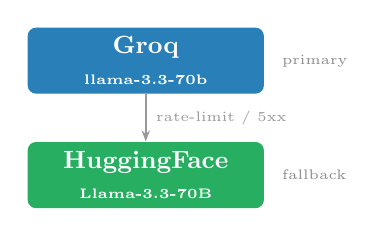
\begin{tikzpicture}[
        box/.style={rectangle, rounded corners=3pt,
                    minimum width=3cm, minimum height=0.65cm,
                    align=center, font=\small\bfseries, text=white},
        arr/.style={-{Stealth[length=4pt]}, thick, color=black!40}
      ]
        \node[box, fill=aims-lblue] (g) {Groq\\{\tiny llama-3.3-70b}};
        \node[box, fill=aims-green, below=0.6cm of g] (h)
              {HuggingFace\\{\tiny Llama-3.3-70B}};
        \draw[arr] (g) -- node[right, font=\tiny\color{black!45}]
              {rate-limit / 5xx} (h);
        \node[font=\tiny\color{black!45}, right=0.1cm of g] {primary};
        \node[font=\tiny\color{black!45}, right=0.1cm of h] {fallback};
      \end{tikzpicture}
      \end{center}
      {\small Controlled by \code{LLM\_PROVIDER=auto}.
      A second key \code{GROQ\_API\_KEY\_2} extends rate-limit headroom.}

    \column{0.52\textwidth}
      \textbf{\color{aims-blue}Chat helpers (used by all agents)}
\begin{lstlisting}[style=pycode]
# Plain text response
chat(client, system, user) -> str

# JSON response (parsed + fallback)
chat_json(client, system, user) -> list | dict
\end{lstlisting}
      \begin{itemize}
        \item Retries with backoff on 429 / 5xx
        \item Provider fallback built into \code{chat()}
        \item JSON fence stripping via \code{extract\_json()}
        \item Empty list returned on JSON parse failure
      \end{itemize}
  \end{columns}
\end{frame}

% ── 9. Backend Architecture ───────────────────────────────────────────────────
\begin{frame}{Backend Architecture}
  \begin{columns}[T]
    \column{0.50\textwidth}
      \textbf{\color{aims-blue}Request lifecycle}
      \begin{enumerate}
        \item \code{POST /api/research} --- validates question, creates job
        \item Returns \code{job\_id} immediately (HTTP 202)
        \item Background thread starts pipeline
        \item Client polls \code{GET /api/research/\{id\}} or\\
              streams via SSE \code{/\{id\}/events}
        \item Final \code{SharedState} persisted to SQLite
      \end{enumerate}
    \column{0.46\textwidth}
      \begin{block}{SQLite WAL mode --- 3 tables}
        \scriptsize
        \code{jobs} --- status, timestamps, score summary\\[0.2em]
        \code{events} --- append-only per-job event log\\[0.2em]
        \code{states} --- full \code{SharedState} JSON blob
      \end{block}
      \vspace{0.4em}
      \begin{block}{In-memory write-through cache}
        \scriptsize
        Job objects cached in a dict for fast SSE polling ---
        written through to SQLite on every update to survive restarts.
      \end{block}
  \end{columns}
\end{frame}

% ── 10. REST API ──────────────────────────────────────────────────────────────
\begin{frame}[fragile]{REST API}
  {\small All \code{/api/research/*} endpoints require \code{X-API-Key} header
  (if \code{API\_KEY} env var is set).}
  \vspace{0.4em}
  \begin{center}
  \small
  \begin{tabular}{lll}
    \toprule
    \textbf{Method} & \textbf{Endpoint} & \textbf{Description} \\
    \midrule
    \textsc{post}   & \code{/api/research}                   & Submit question --- returns \code{job\_id} (202) \\
    \textsc{get}    & \code{/api/research/\{id\}}            & Poll status, report \& evaluation scores \\
    \textsc{get}    & \code{/api/research/\{id\}/events}     & Server-Sent Events live progress stream \\
    \textsc{get}    & \code{/api/research/\{id\}/reasoning}  & Queries, sources, themes (full detail) \\
    \textsc{get}    & \code{/api/research/\{id\}/pdf}        & Download report as PDF \\
    \textsc{delete} & \code{/api/research/\{id\}}            & Delete a single job \\
    \textsc{get}    & \code{/api/health}                     & Health check (no auth required) \\
    \bottomrule
  \end{tabular}
  \end{center}
  \vspace{0.3em}
\begin{lstlisting}[style=shcode]
curl -X POST http://localhost:8000/api/research \
  -H "X-API-Key: your-key" -H "Content-Type: application/json" \
  -d '{"question": "Trade-offs between CNNs and ViTs for medical imaging?"}'
\end{lstlisting}
\end{frame}

% ── 11. Frontend ──────────────────────────────────────────────────────────────
\begin{frame}{Frontend}
  \begin{columns}[T]
    \column{0.46\textwidth}
      \textbf{\color{aims-blue}Stack}\\[0.2em]
      Next.js 16 \textbullet\ React 19 \textbullet\ TypeScript\\
      Tailwind CSS v4 \textbullet\ Vercel
      \vspace{0.5em}

      \textbf{\color{aims-blue}Real-time updates}
      \begin{itemize}
        \item SSE stream via a custom \code{useSSE} hook
        \item Progress bar advances through stages
        \item Report rendered as Markdown on completion
        \item PDF download calls \code{/pdf} endpoint
      \end{itemize}
    \column{0.50\textwidth}
      \textbf{\color{aims-blue}Key components}
      \begin{block}{}
        \scriptsize
        \code{ResearchForm} --- question input + submit\\[0.2em]
        \code{JobStatus} --- live stage indicator + spinner\\[0.2em]
        \code{ReportView} --- Markdown renderer with citations\\[0.2em]
        \code{EvaluationCard} --- score visualisation\\[0.2em]
        \code{ReasoningPanel} --- collapsible sources \& themes
      \end{block}
      \vspace{0.3em}
      \sidenote{Set \code{NEXT\_PUBLIC\_API\_URL} and \code{NEXT\_PUBLIC\_API\_KEY} in \code{frontend/.env.local}}
  \end{columns}
\end{frame}

% ── 12. Technology Stack  ──────────────────────────────────────────────────────
\begin{frame}{Technology Stack}
  \begin{center}
  \small
  \begin{tabular}{>{\bfseries}lll}
    \toprule
    Layer & Technology & Role \\
    \midrule
    Backend      & Python 3.11, FastAPI, Uvicorn          & REST API \& SSE server \\
    LLM primary  & Groq --- \code{llama-3.3-70b-versatile}     & Fast inference \\
    LLM fallback & HuggingFace --- \code{Llama-3.3-70B-Instruct} & Rate-limit fallback \\
    Web search   & DuckDuckGo \textbullet\ Tavily (optional) & Source discovery \\
    Scraping     & httpx \textbullet\ BeautifulSoup4         & Full-page content \& images \\
    Validation   & Pydantic v2                             & SharedState schema \\
    Database     & SQLite WAL mode                         & Job \& state persistence \\
    PDF export   & WeasyPrint                              & Markdown $\to$ styled PDF \\
    Frontend     & Next.js 16 \textbullet\ React 19 \textbullet\ Tailwind v4 & Web UI \\
    Hosting (FE) & Vercel                                  & Frontend deployment \\
    Hosting (BE) & Render                                  & Backend API deployment \\
    \bottomrule
  \end{tabular}
  \end{center}
\end{frame}

% ── 13. Demo ──────────────────────────────────────────────────────────────────
\begin{frame}{Demo --- Example Run}
  \textbf{Question:} \emph{``What are the main trade-offs between CNNs and Vision
  Transformers for medical imaging?''}
  \vspace{0.4em}
  \begin{columns}[T]
    \column{0.32\textwidth}
      \begin{block}{Search}
        \centering\small
        \textbf{3 queries \textbullet\ 14 sources}\\[0.2em]
        {\tiny 47 evidence fragments extracted}
      \end{block}
    \column{0.32\textwidth}
      \begin{block}{Synthesis}
        \centering\small
        \textbf{6 themes \textbullet\ 2 contradictions}\\[0.2em]
        {\tiny Performance \textbullet\ Data efficiency \textbullet\ Interpretability \textbullet\ Computational cost \textbullet\ Transfer learning \textbullet\ Hybrid models}
      \end{block}
    \column{0.32\textwidth}
      \begin{block}{Report}
        \centering\small
        \textbf{\textasciitilde2\,100 words \textbullet\ 7 sections}\\[0.2em]
        {\tiny Citations, 1 Mermaid diagram, 2 embedded images}
      \end{block}
  \end{columns}
  \vspace{0.5em}
  \scorebar{Coverage}{0.88}{aims-green}
  \scorebar{Faithfulness}{0.90}{aims-lblue}
  \scorebar{Hallucination rate \ (lower is better)}{0.12}{aims-red}
  \scorebar{Usefulness}{0.85}{aims-purple}
\end{frame}

% ── 14. Key Design Decisions ──────────────────────────────────────────────────
\begin{frame}{Key Design Decisions}
  \begin{columns}[T]
    \column{0.50\textwidth}
      \stagecard{aims-lblue}{Functional agents over classes}{%
        Each agent is a plain \texttt{run(state) → state} function ---
        easy to test, swap, and trace in isolation.}
      \stagecard{aims-green}{Write-through cache}{%
        In-memory dict for fast SSE polling; SQLite as durable store.
        No cache invalidation complexity.}
      \stagecard{aims-orange}{Two-pass report generation}{%
        Outline first, then prose --- gives the LLM a structural
        skeleton to follow, reducing hallucination risk.}
    \column{0.46\textwidth}
      \stagecard{aims-purple}{Multi-provider LLM fallback}{%
        Auto-fallback from Groq to HuggingFace prevents hard failures
        under rate limits during demos.}
      \stagecard{aims-lblue}{Structured JSON at every boundary}{%
        \texttt{chat\_json()} enforces JSON between all agent stages ---
        no free-form text passing.}
      \stagecard{aims-green}{Source deduplication by URL}{%
        Normalised before building References ---
        no duplicate entries in the final report.}
  \end{columns}
\end{frame}

% ── 15. Limitations ───────────────────────────────────────────────────────────
\begin{frame}{Limitations}
  \begin{columns}[T]
    \column{0.50\textwidth}
      \textbf{\color{aims-blue}Current constraints}
      \begin{itemize}
        \item \textbf{Hallucination risk} --- LLM may invent claims; evaluator detects but does not prevent this
        \item \textbf{Open web only} --- paywalled or un-indexed content unavailable
        \item \textbf{Sequential pipeline} --- no parallel agent execution
        \item \textbf{Context window limits} --- large evidence sets are truncated before LLM calls
      \end{itemize}
    \column{0.46\textwidth}
      \textbf{\color{aims-blue}Known issues}
      \begin{itemize}
        \item \textbf{Search quality variance} --- DDG returns fewer relevant results than Tavily
        \item \textbf{Evaluation circularity} --- faithfulness scored against same evidence pool, not external ground truth
        \item \textbf{Rate limits} --- free Groq tiers hit easily; HF fallback adds latency
        \item \textbf{PDF system libs} --- WeasyPrint requires Pango/Cairo beyond pip
      \end{itemize}
  \end{columns}
\end{frame}

% ── 16. Future Work ───────────────────────────────────────────────────────────
\begin{frame}{Future Work}
  \begin{columns}[T]
    \column{0.32\textwidth}
      \begin{block}{Pipeline}
        \begin{itemize}
          \item Parallel search queries
          \item Iterative refinement loop
          \item Citation verification agent
          \item Domain-specific variants
        \end{itemize}
      \end{block}
    \column{0.32\textwidth}
      \begin{block}{Data \& Quality}
        \begin{itemize}
          \item Academic DB connectors\\(arXiv, PubMed)
          \item External fact-checking
          \item Human-in-the-loop approval
          \item Fine-tuned smaller models
        \end{itemize}
      \end{block}
    \column{0.32\textwidth}
      \begin{block}{Platform}
        \begin{itemize}
          \item WebSocket real-time updates
          \item Multi-user job isolation
          \item Scheduled recurring jobs
          \item WhatsApp / email delivery
        \end{itemize}
      \end{block}
  \end{columns}
  \vspace{0.5em}
  \begin{hlbox}
    Architecture is designed for incremental extension: add an agent module
    $\to$ register fields in \code{SharedState} $\to$ insert one call in
    \code{pipeline.py}.
  \end{hlbox}
\end{frame}

% ── 17. Telegram Bot Integration ──────────────────────────────────────────────
\begin{frame}{Telegram Bot Integration}
  \begin{columns}[T]
    \column{0.50\textwidth}
      \textbf{\color{aims-blue}How it works}
      \begin{enumerate}
        \item User sends a research question to the bot
        \item Bot acknowledges and starts a background job
        \item Progress updates sent at each pipeline stage
        \item Final report delivered as chunked messages
        \item Quality scores included in the summary
      \end{enumerate}
      \vspace{0.4em}
      \sidenote{No business verification needed --- bot token from @BotFather is instant.}
    \column{0.46\textwidth}
      \textbf{\color{aims-blue}Architecture}
      \vspace{0.3em}
      \begin{center}
      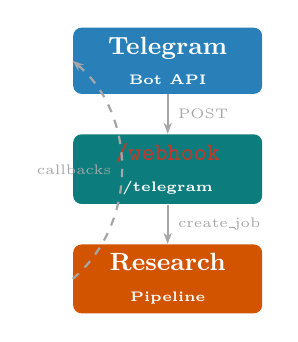
\begin{tikzpicture}[
        box/.style={rectangle, rounded corners=3pt,
                    minimum width=2.4cm, minimum height=0.6cm,
                    align=center, font=\small\bfseries, text=white},
        arr/.style={-{Stealth[length=4pt]}, thick, color=black!35}
      ]
        \node[box, fill=aims-lblue] (tg)  {Telegram\\{\tiny Bot API}};
        \node[box, fill=aims-teal, below=0.5cm of tg] (wh) {\code{/webhook}\\{\tiny /telegram}};
        \node[box, fill=aims-orange, below=0.5cm of wh] (pp) {Research\\{\tiny Pipeline}};
        \draw[arr] (tg) -- node[right, font=\tiny\color{black!45}] {POST} (wh);
        \draw[arr] (wh) -- node[right, font=\tiny\color{black!45}] {create\_job} (pp);
        \draw[arr, dashed] (pp.west) to[bend right=50]
          node[left, font=\tiny\color{black!45}] {callbacks} (tg.west);
      \end{tikzpicture}
      \end{center}
      \vspace{0.3em}
      \begin{block}{}
        \scriptsize
        Reuses existing callback pattern\\
        \code{on\_progress} + \code{on\_complete}\\
        Same as WhatsApp integration
      \end{block}
  \end{columns}
\end{frame}

% ── 18. Deployment ────────────────────────────────────────────────────────────
\begin{frame}[fragile]{Deployment}
  \begin{columns}[T]
    \column{0.50\textwidth}
      \textbf{\color{aims-blue}Backend --- Render}
      \begin{itemize}
        \item Python/FastAPI service on Render free tier
        \item Auto-deploys from \code{main} branch on push
        \item Persistent SQLite volume for job history
        \item Health check on \code{/api/health}
      \end{itemize}
      \vspace{0.4em}
\begin{lstlisting}[style=shcode]
# Set in Render > Environment
GROQ_API_KEY=gsk_...
GROQ_API_KEY_2=gsk_...
HF_API_KEY=hf_...
TAVILY_API_KEY=tvly_...
API_KEY=your-secret
LLM_PROVIDER=auto
\end{lstlisting}

    \column{0.46\textwidth}
      \textbf{\color{aims-blue}Frontend --- Vercel}
      \begin{itemize}
        \item Next.js 16 App Router deployed to Vercel
        \item Points to the Render backend URL
        \item Zero-config CI/CD from Git
      \end{itemize}
      \vspace{0.4em}
      \begin{block}{Vercel env vars}
        \scriptsize
        \code{NEXT\_PUBLIC\_API\_URL}\\
        \hspace{1em}--- Render service URL\\[0.2em]
        \code{NEXT\_PUBLIC\_API\_KEY}\\
        \hspace{1em}--- matches backend \code{API\_KEY}
      \end{block}
      \vspace{0.3em}
      % \begin{center}
      % \begin{tikzpicture}[
      %   box/.style={rectangle, rounded corners=3pt,
      %               minimum width=2.6cm, minimum height=0.55cm,
      %               align=center, font=\small\bfseries, text=white},
      %   arr/.style={-{Stealth[length=4pt]}, thick, color=black!35}
      % ]
      %   \node[box, fill=aims-lblue] (u)  {User\\{\tiny browser}};
      %   \node[box, fill=aims-teal,  right=0.3cm of u] (v)  {Vercel\\{\tiny Next.js}};
      %   \node[box, fill=aims-orange,right=0.3cm of v] (r)  {Render\\{\tiny FastAPI}};
      %   \draw[arr] (u) -- (v);
      %   \draw[arr] (v) -- (r);
      % \end{tikzpicture}
      % \end{center}
  \end{columns}

  \begin{center}
  
\begin{tikzpicture}[
    box/.style={rectangle, rounded corners=3pt,
                minimum width=2.6cm, minimum height=0.55cm,
                align=center, font=\small\bfseries, text=white},
    arr/.style={-{Stealth[length=4pt]}, thick, color=black!35}
  ]
    \node[box, fill=aims-lblue] (u)  {User\\{\tiny browser}};
    \node[box, fill=aims-teal,  right=0.3cm of u] (v)  {Vercel\\{\tiny Next.js}};
    \node[box, fill=aims-orange,right=0.3cm of v] (r)  {Render\\{\tiny FastAPI}};
    \draw[arr] (u) -- (v);
    \draw[arr] (v) -- (r);
  \end{tikzpicture}
  \end{center}
\end{frame}

% ── 19. Conclusion ────────────────────────────────────────────────────────────
\begin{frame}{Conclusion}
  \begin{columns}[T]
    \column{0.50\textwidth}
      \textbf{\color{aims-blue}What we built}
      \begin{itemize}
        \item End-to-end automated research pipeline with 4 specialised AI agents
        \item FastAPI backend: async jobs, SSE streaming, SQLite persistence
        \item Next.js frontend with real-time progress and PDF export
        \item Telegram bot for conversational access
        \item Multi-provider LLM layer with automatic fallback and retries
        \item Built-in self-evaluation on a 4-criterion quality rubric
      \end{itemize}
    \column{0.46\textwidth}
      \textbf{\color{aims-blue}Key takeaways}
      \begin{itemize}
        \item Multi-agent decomposition makes complex tasks tractable and inspectable
        \item Structured JSON at every boundary is essential for reliability
        \item Self-evaluation adds accountability without external ground truth
        \item Provider abstraction is critical for demo reliability under rate limits
      \end{itemize}
      \vspace{0.4em}
      \begin{hlbox}
        Every component is inspectable --- from a single question to a scored, cited report.
      \end{hlbox}
  \end{columns}
\end{frame}

% ── 20. Q\&A ──────────────────────────────────────────────────────────────────
\begin{frame}[plain]
  \begin{center}
    \vfill
    {\Huge\bfseries\color{aims-blue}Thank you}\par
    \vspace{0.4em}
    {\large\color{aims-teal}Questions?}\par
    \vspace{0.7em}
    
\begin{tikzpicture}
      \draw[aims-teal, line width=1.2pt] (0,0) -- (6cm,0);
    \end{tikzpicture}\par
    \vspace{0.7em}
    {\small\color{black!55}
      J.N.\ Mabiala \textbullet\ S.\ Kargbo \textbullet\ C.\ Akyeampong
      \textbullet\ A.\ Nunoo \textbullet\ Lambert\\[0.3em]
      AIMS RIC \textbullet\ Doctoral Training School 2026%
    }\par
    \vspace{0.5em}
    {\footnotesize\color{aims-blue!65}
      FastAPI \textbullet\ Groq / Llama-3.3-70B \textbullet\ Next.js 16
      \textbullet\ Telegram Bot \textbullet\ Pydantic v2 \textbullet\ SQLite WAL
      \textbullet\ Render \textbullet\ Vercel%
    }
    \vfill
  \end{center}
\end{frame}

\end{document}
